Useful tools that allow the development of Android applications are found in the Android \gls{sdk}. It is the case of the \textit{Emulator}, placed at \texttt{tools/} and the \gls{adb}, placed at \texttt{platform-tools/}. This section describes both tools regarding valuable their features to this project.

\subsection{Android Emulator}

Android provides a mobile device emulator based on the QEMU virtual machine, that runs on the computer. This Emulator provides a real Android environment, being able to run any application. It is very useful to developers, because avoids the need of having a real device in order to run applications. However, depending on the computer, the performance of the Android Emulator may be considerable low when compared to a real devices.

\begin{figure}[h]
 \centering
 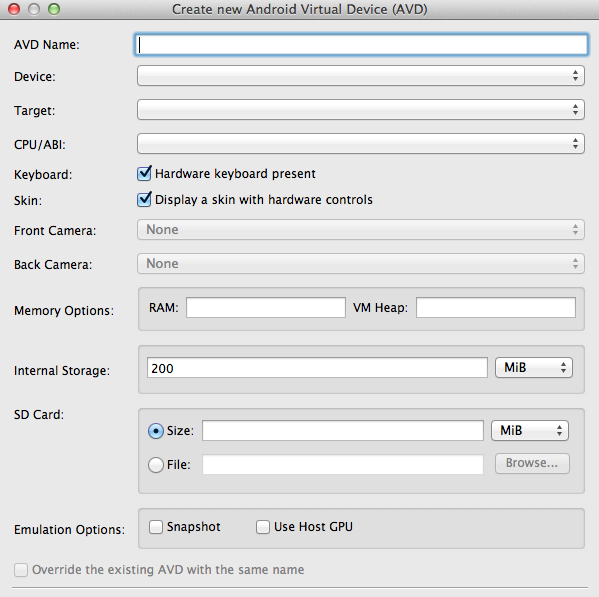
\includegraphics[scale=0.5]{figures/avd.png}
 \caption{Android Virtual Device configuration}
 \label{fig:avd}
\end{figure}

The Android Emulator boots an Android image according to the \gls{avd} configuration file. The \gls{avd} allows to define hardware and software characteristics of a specific model to run on the Android Emulator. \autoref{fig:avd} shows a snapshot of the \gls{AVD} window configuration. For instance, in the \textit{Device} option it is possible to choose an Android model, as \textit{Nexus 4}, \textit{Nexus 7}, \textit{Nexus 10}, \textit{Galaxy Nexus}, \textit{Nexus S}, etc. The \textit{Target} element defines the Android version and the corresponding \gls{api}, as \textit{Android 2.3.3 - API Level 10}, \textit{Android 4.4 - API Level 19}, etc.

Once the \gls{avd} is created, the Emulator may be launched through the \gls{avd} Manager or using the command line. This last provides more options and fits better our needs when developing DroidGuardian. Some useful commands are presented as follow:


\begin{lstlisting}[style=BashInputStyle]
# emulator -avd <avd_name>
\end{lstlisting}

This command launches the Emulator with the \gls{avd} image called \textt{avd\_name}. \gls{svd} files are usually stored at \texttt{.android/avd/} within the Android \gls{sdk} folder.

\begin{lstlisting}[style=BashInputStyle]
# emulator -avd <avd_name> -kernel <kernel_path>
\end{lstlisting}

In order to choose a kernel of our own to run on the Emulator, it is used the \textit{kernel} flag providing the image file system path of the kernel.

 \begin{lstlisting}[style=BashInputStyle]
# emulator -avd <avd_name> -kernel <kernel_path> - show-kernel -verbose
\end{lstlisting}

To follow what is happening during the boot and to inspect the kernel prints, the Emulator provides both \textit{show-kernel} and \textit{verbose} flags.

\subsection{Android Debug Bridge}

\gls{adb} is another useful tool that connects the computer to Android devices (real or emulated). This connection brings powerful features that will be described in this section. The \gls{adb} tool, mention as adb from now on, is available as a command line. It is a client-server program that comprises three components:

\begin{itemize}
\item A client, that runs on the development computer;
\item A server, that runs as a background process on the development computer. The server handles communication between the client and the daemon;
\item A daemon, that runs in background on the mobile device (real or emulated).
\end{itemize}

Once we start an Android Emulator, this becomes available to connection through adb. The following command shows all Android devices running on the computer:

 \begin{lstlisting}[style=BashInputStyle]
# adb devices
\end{lstlisting}

If we have one Android Emulator running on the computer, the output returned is the following:

 \begin{lstlisting}[style=BashInputStyle]
List of devices attached 
emulator-5554	device
\end{lstlisting}

With adb it is possible to:

\begin{itemize}

\item install an Android application on the emulator/device;
 \begin{lstlisting}[style=BashInputStyle]
# adb install <path_to_apk>
\end{lstlisting}

\item copy a specified file from the emulator/device to the development computer;
 \begin{lstlisting}[style=BashInputStyle]
# adb pull <remote> <local>
\end{lstlisting}

\item copy a specified file from the development computer to the emulator/device;
 \begin{lstlisting}[style=BashInputStyle]
# adb push <local> <remote>
\end{lstlisting}

\item print the logcat output;
 \begin{lstlisting}[style=BashInputStyle]
# adb logcat
\end{lstlisting}

\item start a remote shell in the target emulator/device:
 \begin{lstlisting}[style=BashInputStyle]
# adb shell
\end{lstlisting}

\end{itemize}

There are more operations and options to perform with adb, that can be checked on the Android online page\footnote{http://developer.android.com/tools/help/adb.html}.